\section*{Supplementary Material}

\begin{center}
	\vspace*{1cm} % Force vertical space below header
	\textbf{\LARGE 		Omnisoot: an object-oriented computational package for the simulation of the gas phase synthesis of Carbon Black} 
\end{center}

\begin{center}
	Mohammad Adib$^{1,*}$, Sina Kazemi$^1$, M. Reza Kholgy$^{1,*}$ \\
	{\small *Corresponding author} \\
	$^1$ Department of Mechanical and Aerospace Engineering, Carleton University, 1125 Colonel By Dr, Ottawa, ON K1S 5B6, Canada
\end{center}

\beginsupplement


\section{Gas scrubbing rates}
\label{sec:gasscrub}

The rate of production/destruction of species involved in soot formation must be taken into account to preserve the mass and energy balance in reactive systems. In order to do that, the production rate of gaseous species calculated by Cantera must be corrected for the rate of release/consumption due to PAH growth and surface reaction models calculated in the previous sections.

\begin{equation}
	\left(
	\frac{d\left[{\mathrm{PAH_j}}\right]}{dt}
	\right)_{tot}
	= 
	\left(
	\frac{d\left[{\mathrm{PAH_j}}\right]}{dt}
	\right)_{gas}
	+
	\left(
	\frac{d\left[{\mathrm{PAH_j}}\right]}{dt}
	\right)_{inc}
	+
	\left(
	\frac{d\left[{\mathrm{PAH_j}}\right]}{dt}
	\right)_{ads}
	\label{eqn:PAHscrub_total}.
\end{equation}

$\mathrm{H_2}$ is released to the gas mixture due to inception, PAH adsorption as well as oxidation.

\begin{equation}
	\left(
	\frac{d\left[{\mathrm{H_2}}\right]}{dt}
	\right)_{tot}
	= 
	\left(
	\frac{d\left[{\mathrm{H_2}}\right]}{dt}
	\right)_{gas}
	+
	\left(
	\frac{d\left[{\mathrm{H_2}}\right]}{dt}
	\right)_{inc}
	+
	\left(
	\frac{d\left[{\mathrm{H_2}}\right]}{dt}
	\right)_{ads}
	+
	\left(
	\frac{d\left[{\mathrm{H_2}}\right]}{dt}
	\right)_{ox}
	\label{eqn:H2scrub_total}.
\end{equation}

Surface growth consumes $\mathrm{C_2H_2}$ and adds $\mathrm{H_2}$ to the gas mixture.

\begin{equation}
	\left(
	\frac{d\left[{\mathrm{C_2H_2}}\right]}{dt}
	\right)_{tot}
	= 
	\left(
	\frac{d\left[{\mathrm{C_2H_2}}\right]}{dt}
	\right)_{gas}
	+
	\left(
	\frac{d\left[{\mathrm{C_2H_2}}\right]}{dt}
	\right)_{gr}
	\label{eqn:C2H2scrub_total}.
\end{equation}


\begin{equation}
	\left(
	\frac{d\left[{\mathrm{H}}\right]}{dt}
	\right)_{tot}
	= 
	\left(
	\frac{d\left[{\mathrm{H}}\right]}{dt}
	\right)_{gas}
	+
	\left(
	\frac{d\left[{\mathrm{H}}\right]}{dt}
	\right)_{gr}
	\label{eqn:Hscrub_total}.
\end{equation}

Oxidation uses $\mathrm{O_2}$ and $\mathrm{OH}$ to remove carbon from soot particles and generates $\mathrm{H_2}$ and $\mathrm{CO}$.

\begin{equation}
	\left(
	\frac{
		d\left[
		\mathrm{CO}
		\right]
	}{dt}
	\right)_{tot}
	= 
	\left(
	\frac{d\left[{\mathrm{CO}}\right]}{dt}
	\right)_{gas}
	+
	\left(
	\frac{d\left[{\mathrm{CO}}\right]}{dt}
	\right)_{ox}
	\label{eqn:COscrub_total}.
\end{equation}

\begin{equation}
	\left(
	\frac{
		d\left[
		\mathrm{O2}
		\right]
	}{dt}
	\right)_{tot}
	= 
	\left(
	\frac{d\left[{\mathrm{O2}}\right]}{dt}
	\right)_{gas}
	+
	\left(
	\frac{d\left[{\mathrm{O2}}\right]}{dt}
	\right)_{ox}
	\label{eqn:O2scrub_total}.
\end{equation}

\begin{equation}
	\left(
	\frac{
		d\left[
		\mathrm{OH}
		\right]
	}{dt}
	\right)_{tot}
	= 
	\left(
	\frac{d\left[{\mathrm{OH}}\right]}{dt}
	\right)_{gas}
	+
	\left(
	\frac{d\left[{\mathrm{OH}}\right]}{dt}
	\right)_{ox}
	\label{eqn:OHscrub_total}.
\end{equation}

\section{The Effect of Formation and Sensible Energy of Soot}

\begin{figure}[H]
	\centering
	\begin{subfigure}[t]{0.43\textwidth}
		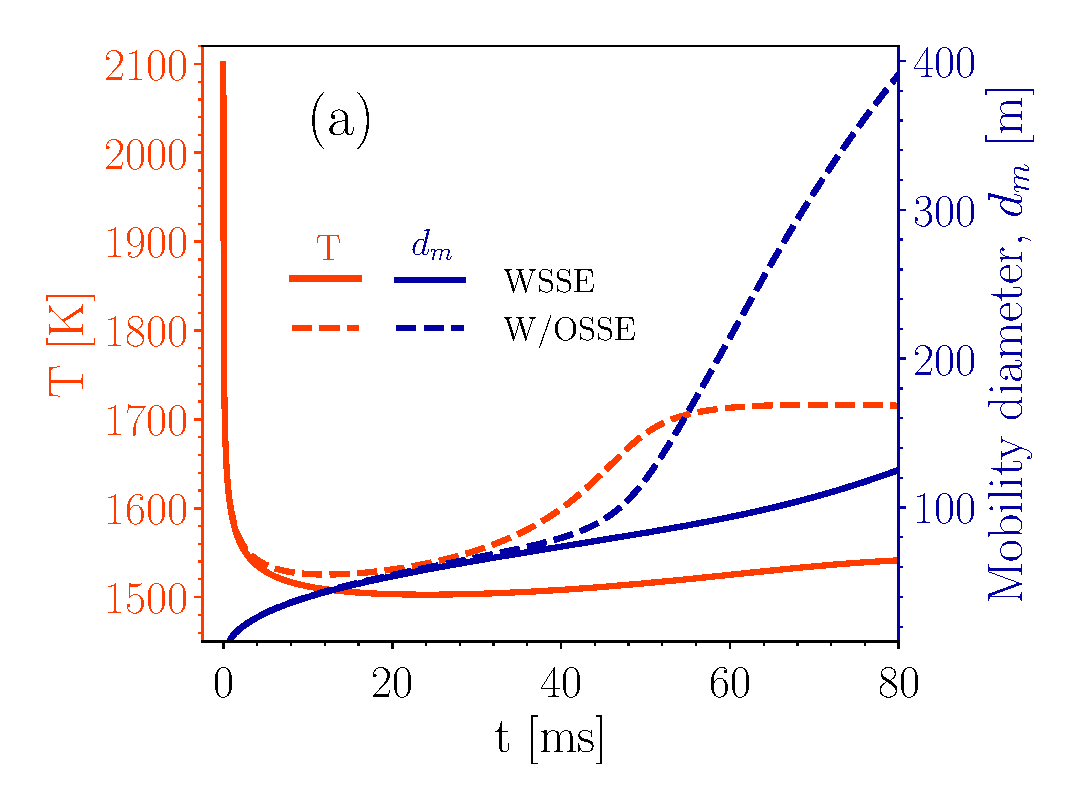
\includegraphics[width=1\textwidth]{Figures/Theory/sse_temp_dm.pdf}
	\end{subfigure}
	\begin{subfigure}[t]{0.4\textwidth}
		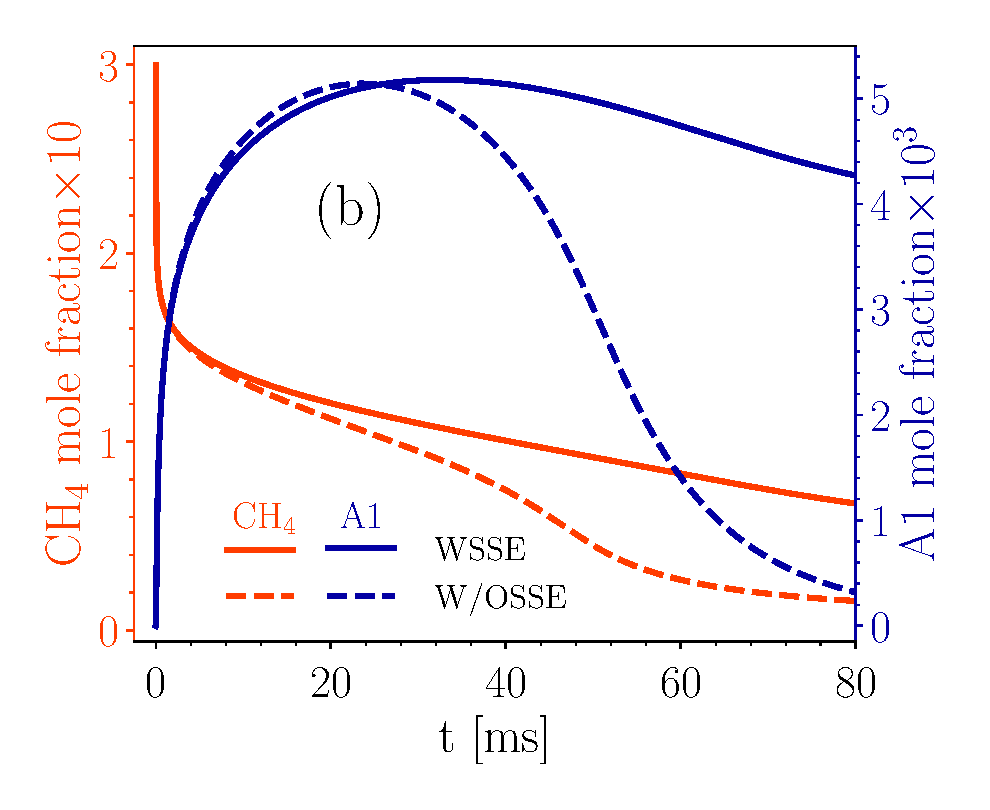
\includegraphics[width=1\textwidth]{Figures/Theory/sse_gasresid.pdf}
	\end{subfigure}
	\caption{The comparison of temperature and soot mobility diameter, $d_m$ (a) and the mole fraction of methane, $\mathrm{CH_4}$, and benzene, A1 in the simulation of the pyrolysis of 30\%$\mathrm{CH_4}$-Ar when soot sensible energy is considered (labeled as ``WSSE") and neglected (labeled as ``W/OSSE"). The constant volume reactor is used along with Caltech mechanism~\citep{blanquart2009chemical}, Reactive Dimerization and the monodisperse population balance model}
	\label{fig:sseeffect}
\end{figure}

\section{Validation of Mass and Energy Balance}

\subsubsection{Constant Volume Reactor}
The pyrolysis of 30\% $\mathrm{CH_4}$ diluted in $\mathrm{N_2}$ with the initial temperature and pressure of 2455 K and 3.47 atm, respectively, was simulated using CVR model for the residence time of 40 ms. The combination of available PAH growth and particle dynamics models leads to eight different cases that were simulated to ensure the conservation of mass and energy. Here, we focus on the total elemental balance of carbon and hydrogen because they are involved in soot processes. 
Figure~\ref{fig:constuvvalid} demonstrates the relative error of total carbon, hydrogen and energy of system for different PAH growth and particle dynamics models in the constant pressure reactor that is less than $\mathrm{10^{-10}}$ for all parameters confirming the validity of model in satisfying the mass and energy balance.

\begin{figure}[H]
	\centering
	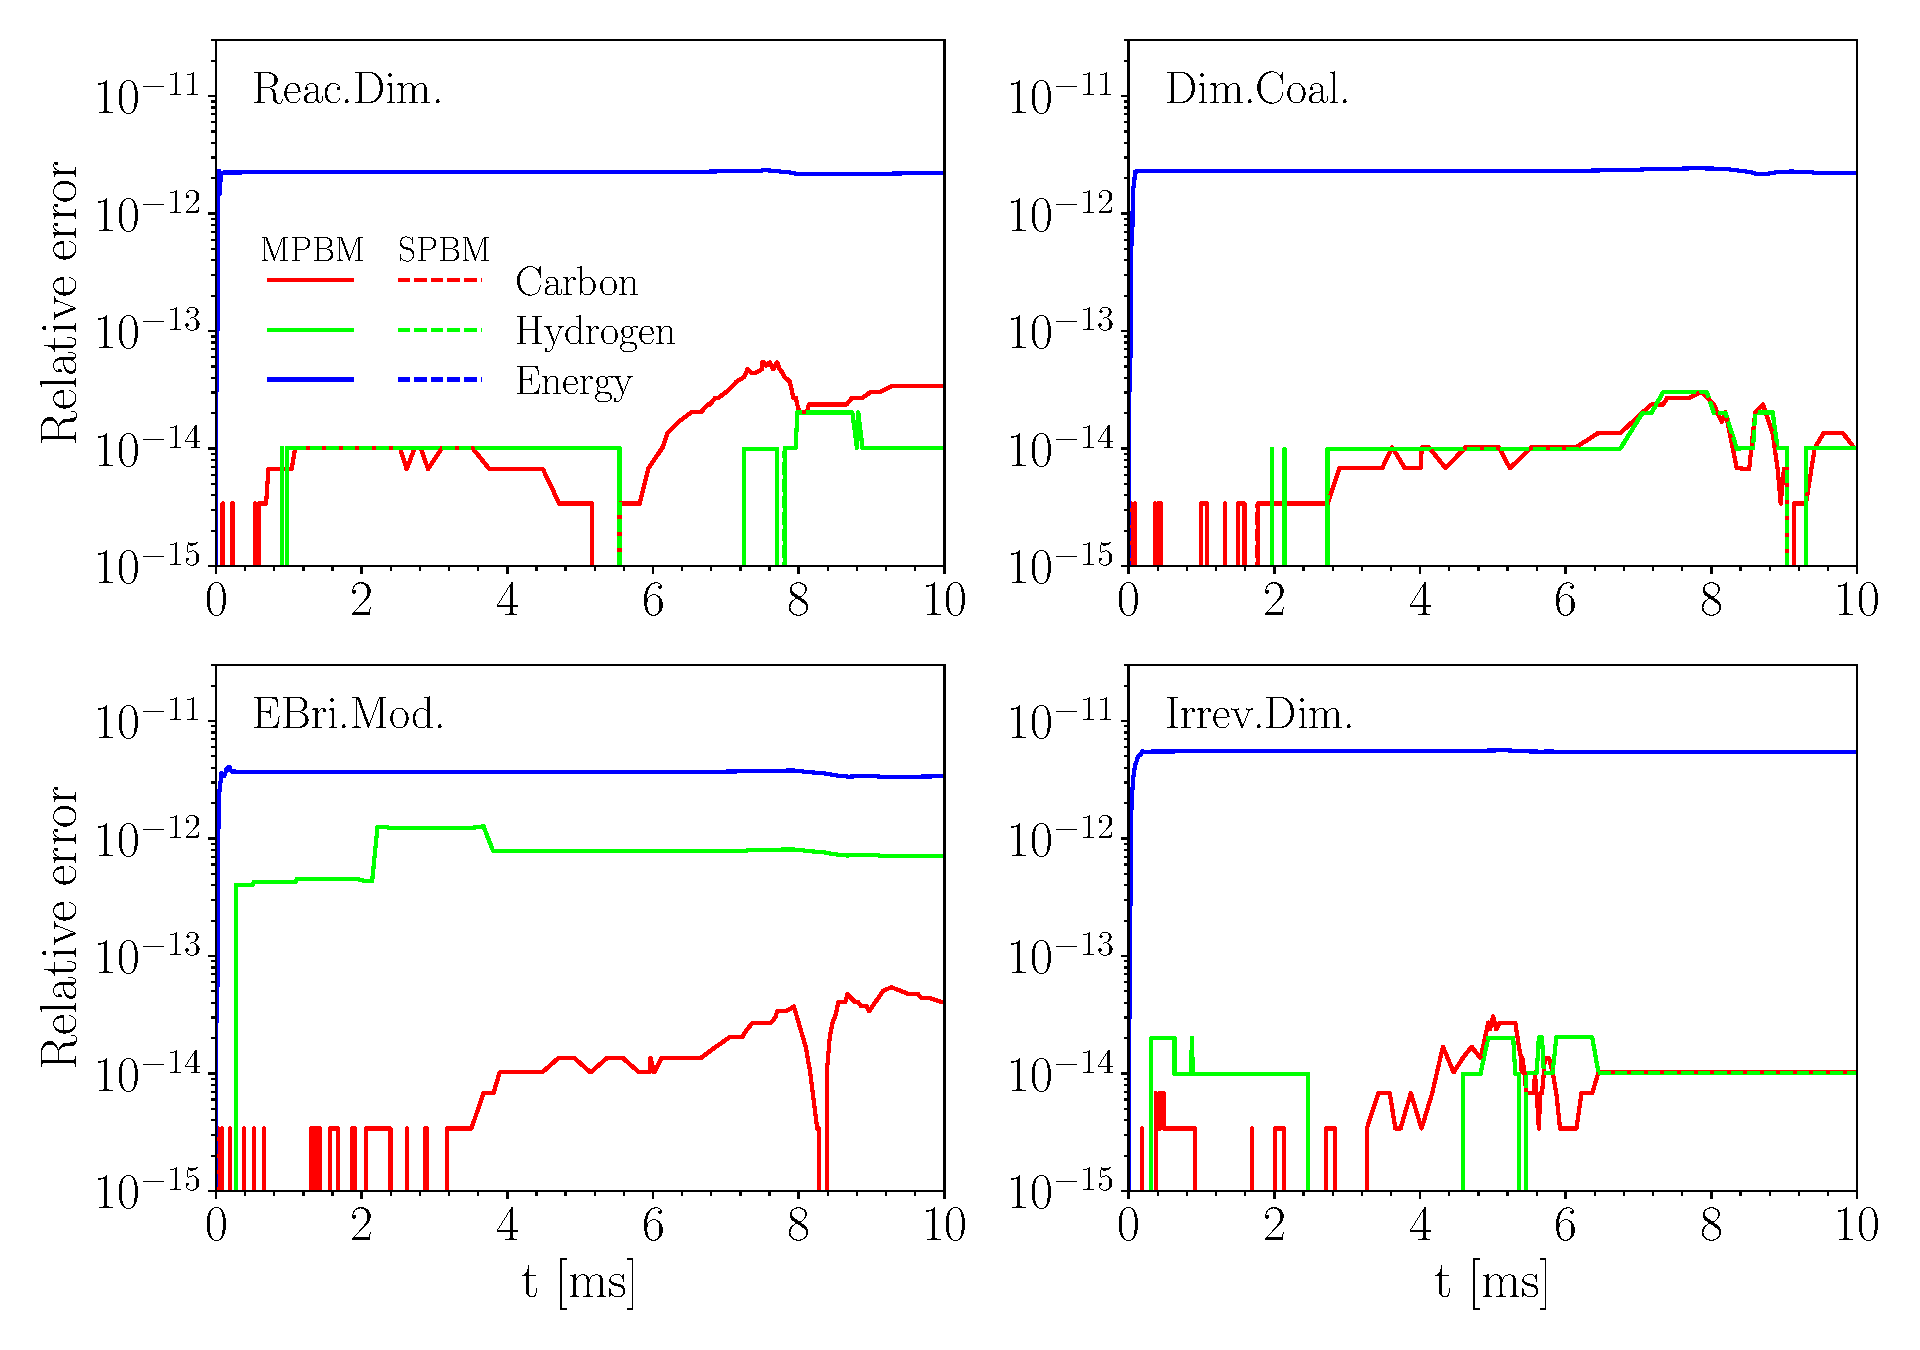
\includegraphics[width=0.8\textwidth]{Figures/Results/Validation/ConstUV/relerr_constuv.pdf}
	\caption{The relative error (residual) of total carbon (red line) and hydrogen (green line) mass, and total internal energy residual of gas and soot (blue line) plotted against residence time during pyrolysis of 30\% $\mathrm{CH_4}$-$\mathrm{N_2}$ at 2455 K and 3.47 atm in CVR simulated using different PAH growth models along with MPBM (solid line) and SPBM (dashed line).}
	\label{fig:constuvvalid}
\end{figure}


\subsection{Constant Pressure Reactor}

The pyrolysis of 5\% $\mathrm{CH_4}$-Ar in a shock-tube with post-reflected-shock temperature and pressure of $\mathrm{T_5}=$2355 K and $\mathrm{P_5}=$4.64 atm, respectively, was simulated using CPR model. Figure~\ref{fig:cprvalid} shows the relative error of total carbon, hydrogen and energy of system for different PAH growth and particle dynamics models in the constant volume that falls below $\mathrm{10^{-10}}$ for all parameters confirming the validity of model in satisfying the mass and energy balance in the constant pressure reactor using all models.

\begin{figure}[H]
	\centering
	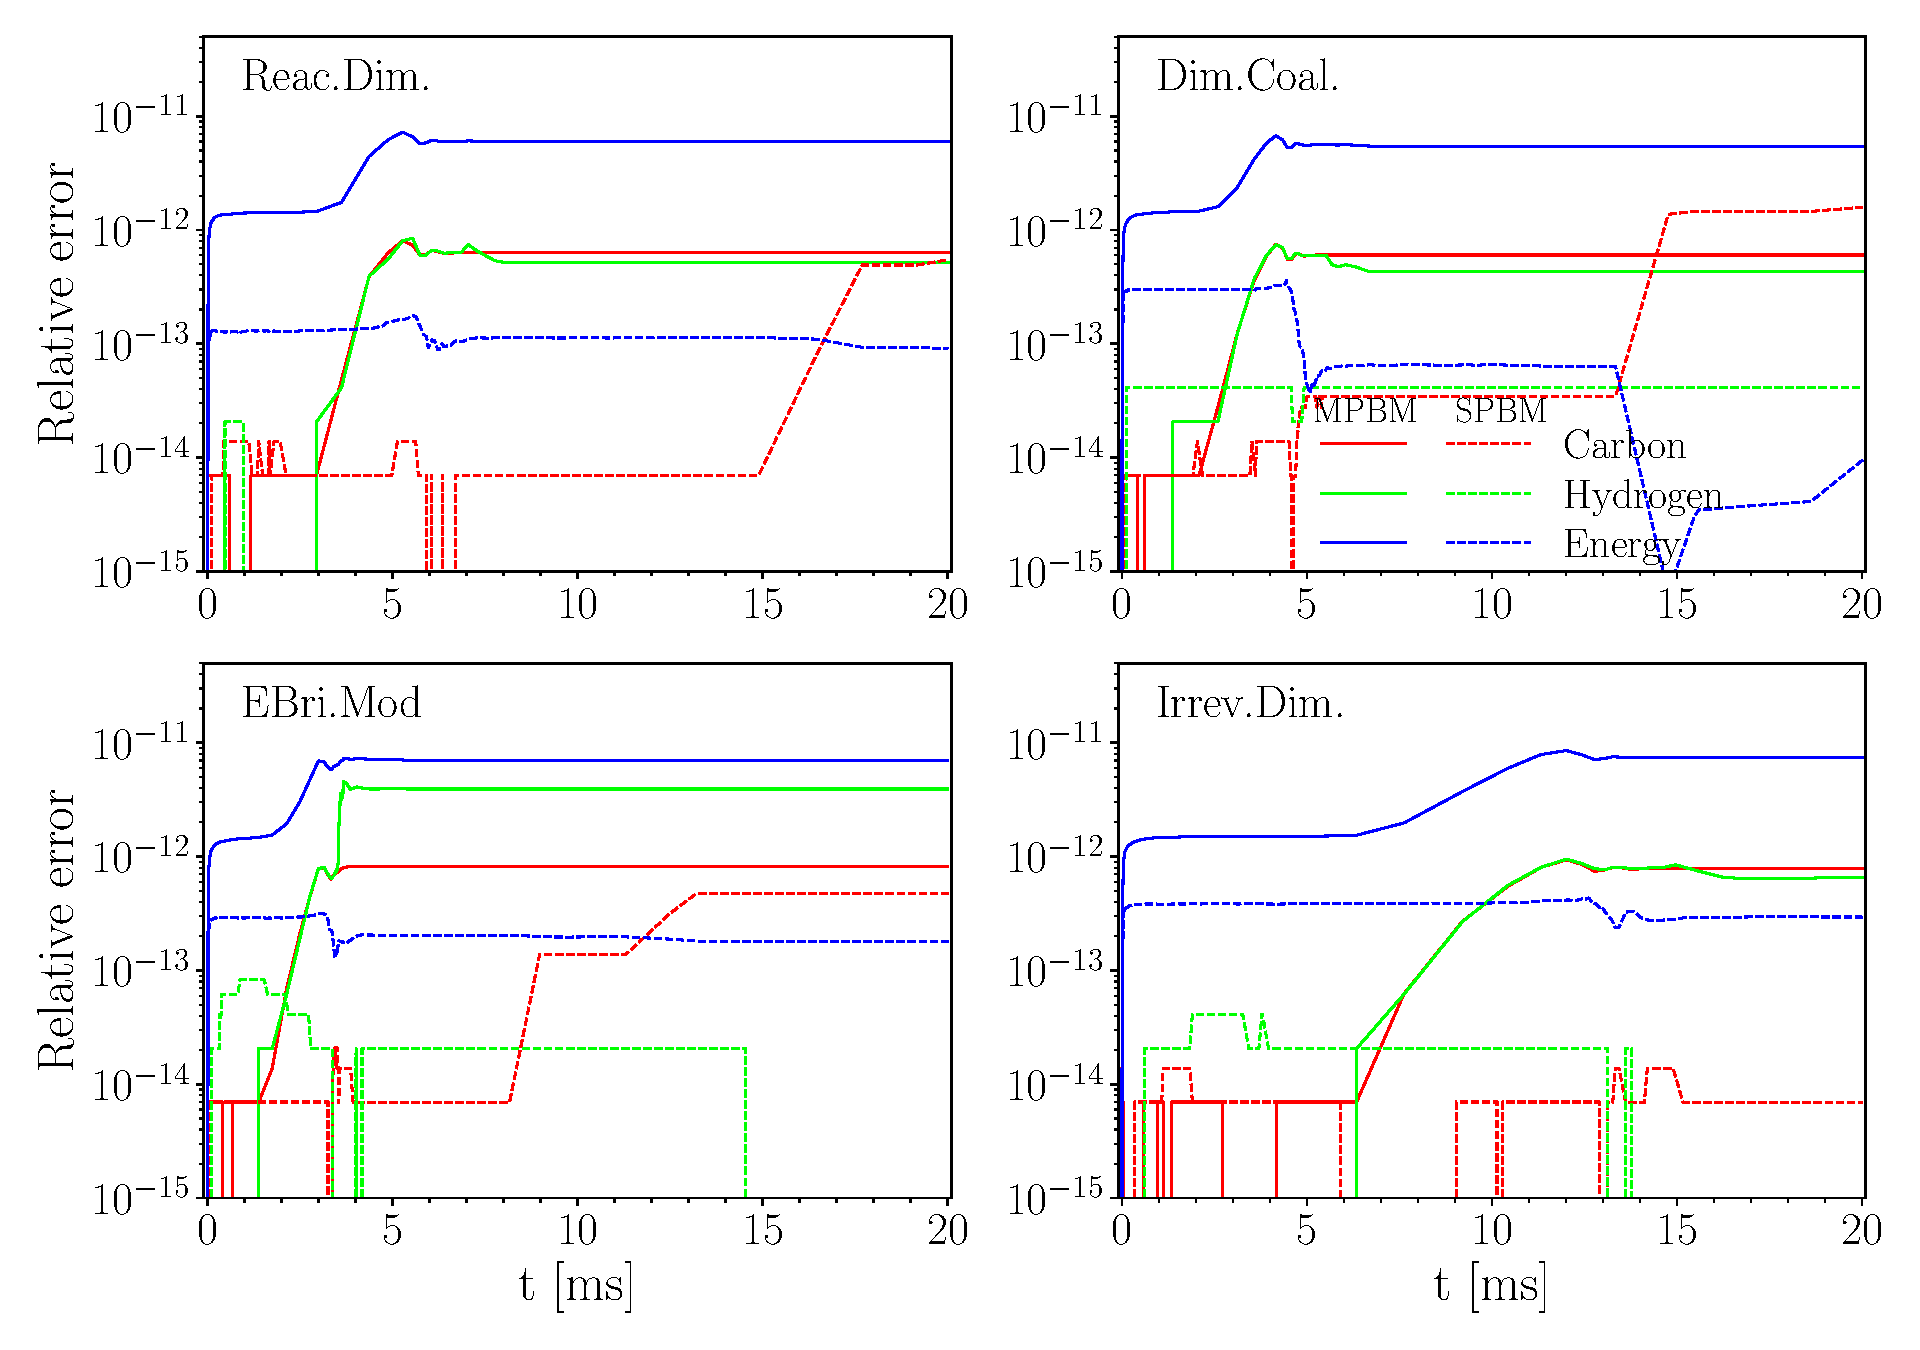
\includegraphics[width=0.8\textwidth]{Figures/Results/Validation/CPR/relerr_cpr.pdf}
	\caption{The relative error (residual) of total carbon (red line) and hydrogen (green line) mass, and total internal energy residual of gas and soot (blue line) plotted against residence time during pyrolysis of 5\% $\mathrm{CH_4}$-Ar at 2355 K and 4.64 atm simulated using CPR with different combinations of PAH growth models and particle dynamics models: MPBM (solid line) and SPBM (dashed line).}
	\label{fig:cprvalid}
\end{figure}

\subsection{Perfectly Stirred Reactor}
\label{sec:psrvalid}
The mass and energy balance are investigated for soot formation during ethylene-air oxidation at equivalence ratio, $\phi=2$ in a perfectly stirred reactor. The simulation conditions were chosen based on the combustor implemented and utilized by \citet{stouffer2002combustion}. The reactants initially at 300 K enter a reactor of 250 ml that works under atmospheric pressure. The simulation is initialized from a high temperature ($\approx$2000 K) to avoid trivial solution (cold reactant leaving the reactor with no chemical reactions) and to ensure the model captures a sustained combustion. The residence time of products in the reactor is 8.5 ms. Figure~\ref{fig:psrvalid} shows the relative error of total elemental carbon and hydrogen mass and total enthalpy of gas and soot, which is less than $10^{-6}$ for all combinations of particle dynamics and PAH growth models.

\begin{figure}[H]
	\centering
	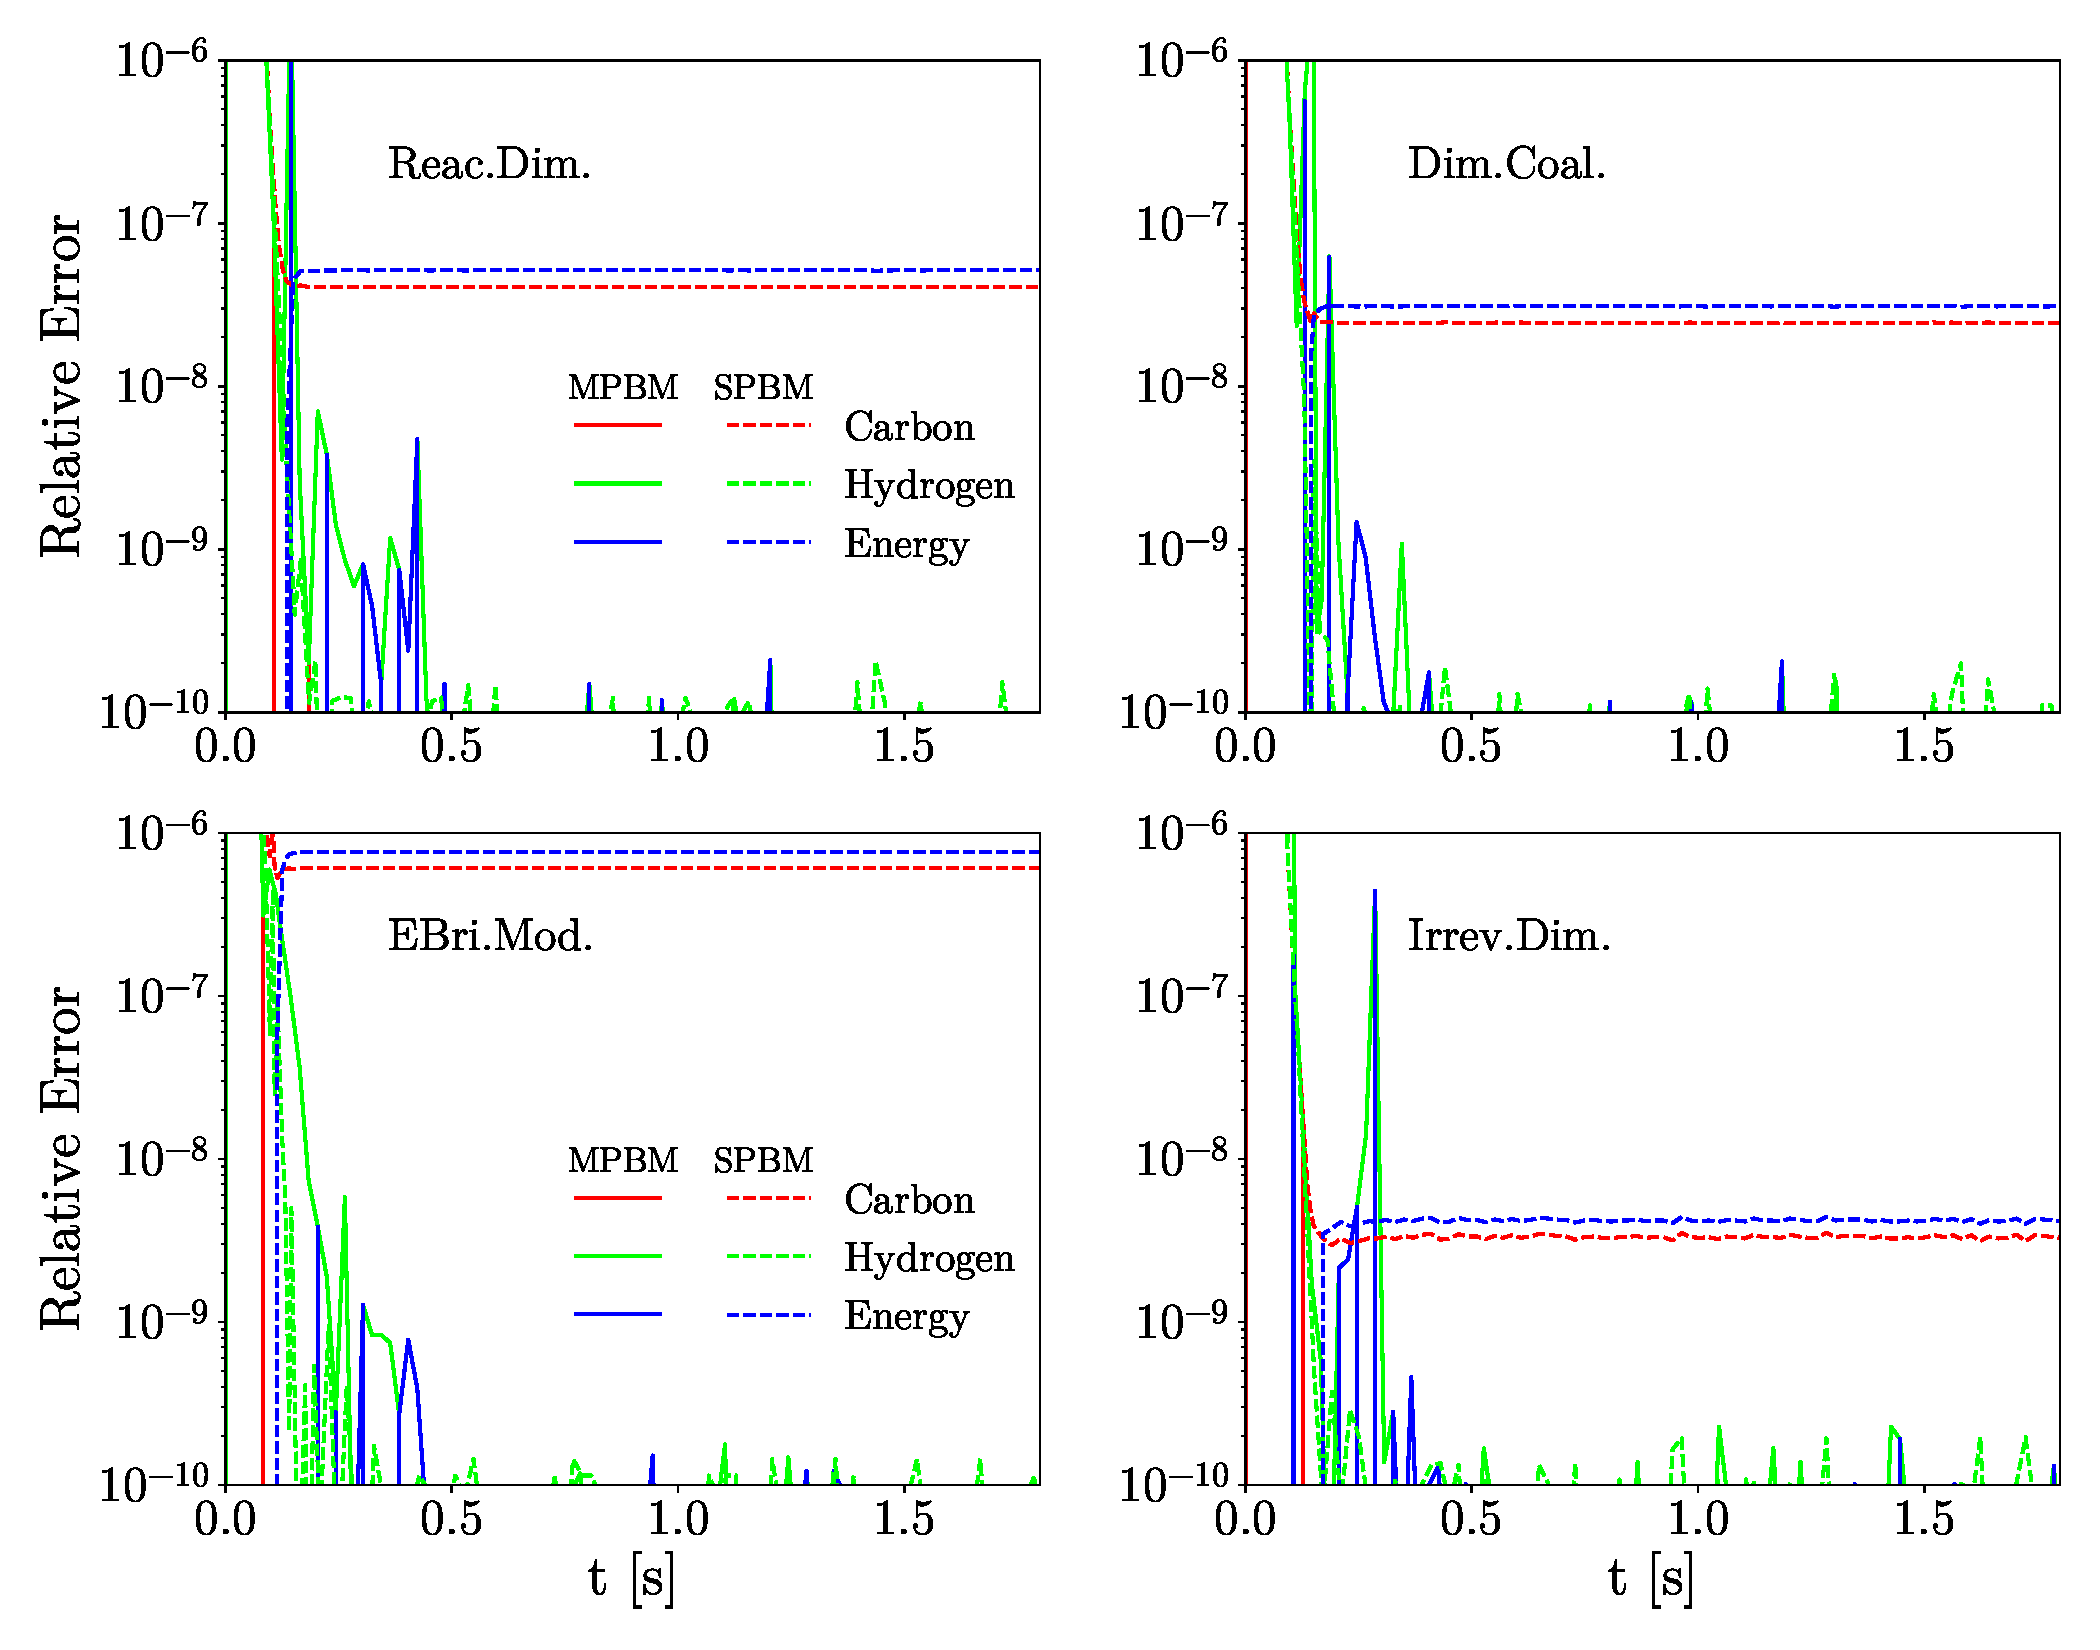
\includegraphics[width=0.8\textwidth]{Figures/Results/Validation/PSR/relerr_psr.pdf}
	\caption{The relative error (residual) of total carbon (red line) and hydrogen (green line) mass, and total internal energy residual of gas and soot (blue line) plotted in simulation time during adiabatic combustion of $\mathrm{C_2H_4}$-air with $\phi=2$ at 1 atm simulated using different combinations of PAH growth models and particle dynamics models: MPBM (solid line) and SPBM (dashed line).}
	\label{fig:psrvalid}
\end{figure}


\subsection{Plug Flow Reactor}
Methane pyrolysis in an adiabatic flow reactor is used to check elemental carbon and hydrogen, and energy balance in the PFR model. The inlet flow enters the reactor at the composition of 30\% $\mathrm{CH_4}$ diluted in $\mathrm{N_2}$, and $T=$2100 K and $P=$1 atm. Figure~\ref{fig:pfrvalid} shows the residual of total elemental carbon and hydrogen, and energy up to 40 cm of the reactor length using all PAH growth and particle dynamics models. The residuals are in the order of $10^{-11}$ and start to grow at the beginning of the reactor by pyrolysis of $\mathrm{CH_4}$ and the formation of intermediate species such and $\mathrm{C_2H_2}$ and PAHs. This initiates soot inception and surface growth affecting the gas chemistry and energy that ends near $z=$10 cm, and then the coagulation of particles is dominant with no a=effect on mass and energy of particles. As a result, PFR model of omnisoot satisfies the conservation of the mass and energy.


\begin{figure}[H]
	\centering
	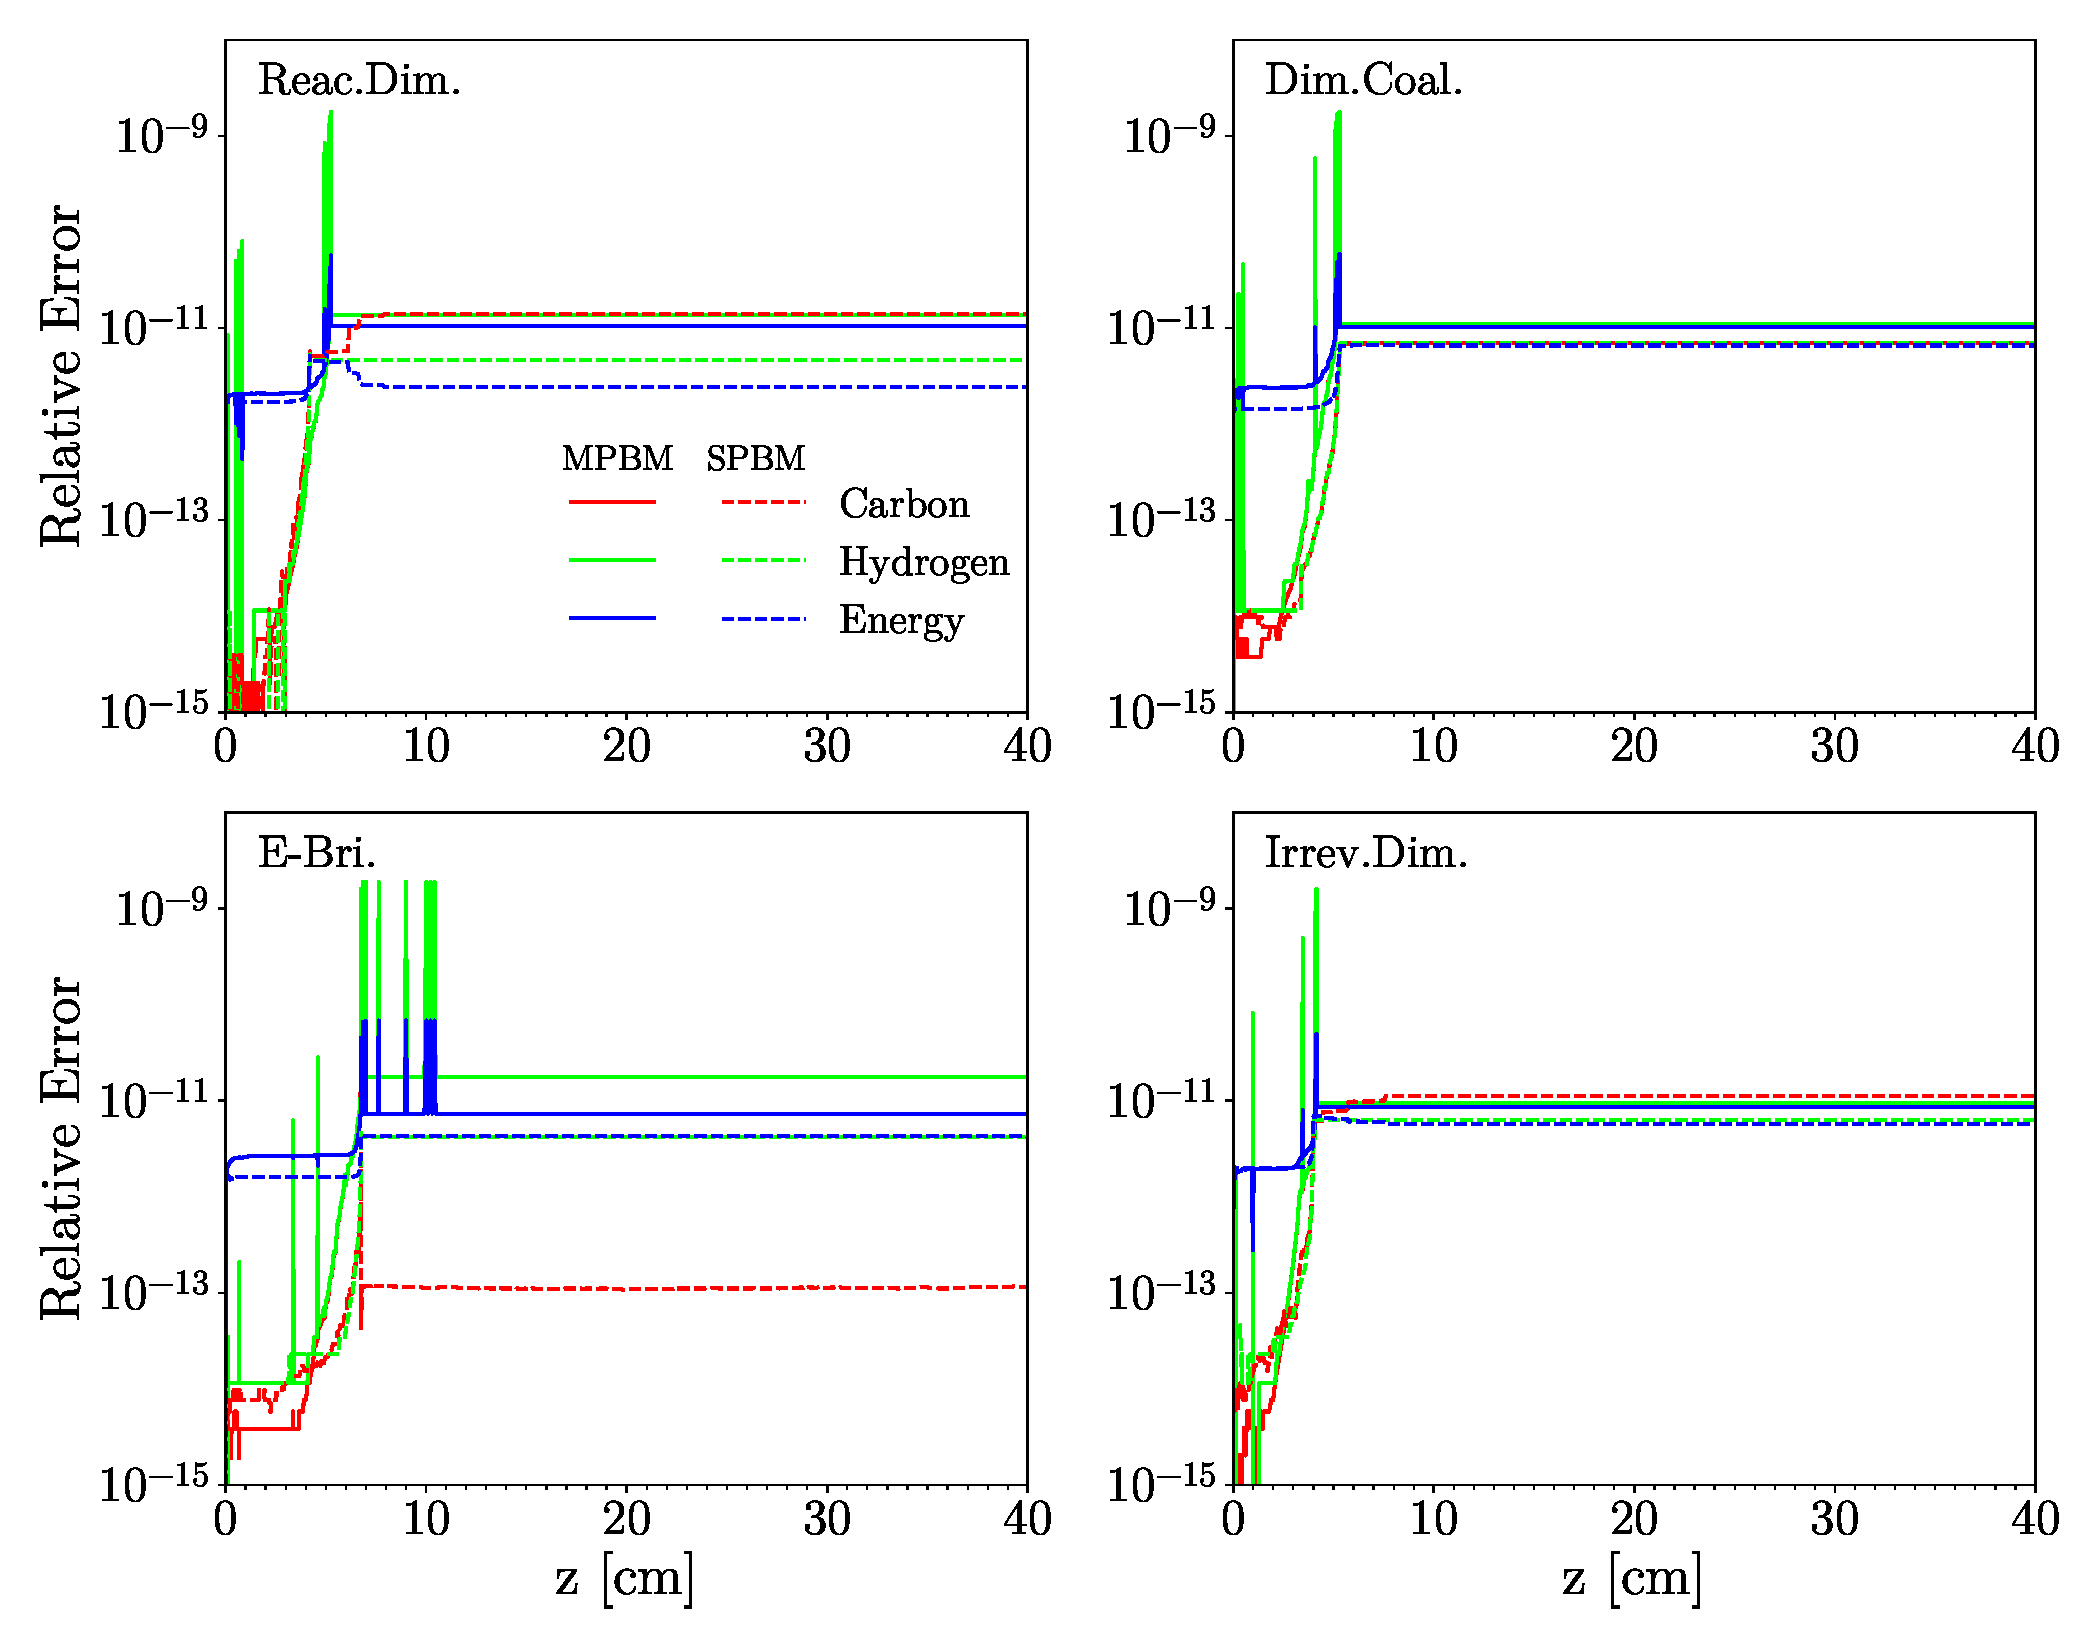
\includegraphics[width=0.8\textwidth]{Figures/Results/Validation/PFR/relerr_pfr.pdf}
	\caption{The relative error (residual) of total carbon (red line) and hydrogen (green line) mass, and total internal energy residual of gas and soot (blue line) plotted against reactor length (cm) in the adiabatic flow reactor during pyrolysis of 30\% $\mathrm{CH_4}$-$\mathrm{N_2}$ at 2100 K and 1 atm simulated using different combinations of PAH growth models and particle dynamics models: MPBM (solid line) and SPBM (dashed line).}
	\label{fig:pfrvalid}
\end{figure}


\section{Validation Collision Frequency}
The collision frequency function determines the rate at which two particles collide, which results in the reduction of total number of agglomerates and increase in size. In the absence of strong flow shear or external forces, Brownian motion is the main driving force for particle coagulation. As explained in Sections~\ref{sec:monocoag} and \ref{sec:sectcoag}, omnisoot employs harmonic mean and Fuchs interpolations to calculate collision frequency of agglomerates from free-molecular to continuum regimes based on gas mean free path and particle morphology. 

The test case for validation of collision frequency is based on the DEM simulation of 2000 monodisperse spherical particles with the density of 2200 $\mathrm{kg/m^3}$ in
a cubic cell with the constant temperature of 298 K and pressure of 1 atm~\citep{goudeli2015coagulation}. Figure~\ref{fig:kernelvalid} depicts the collision frequency plotted against Knudsen number (Kn$=2\lambda/d_m$) obtained by omnisoot using harmonic mean (red solid line) and Fuchs interpolation (green dashed line) and DEM results of \citet{goudeli2015coagulation}. The Fuchs interpretation perfectly matches DEM data over the free-molecular (Kn$<$10) to the continuum (Kn$>$10) range. Harmonic mean is also in good agreement with the DEM results in the free-molecular and continuum regime, but slightly underpredicts the collision frequency in the transition regime (0.1$\le$Kn$\le$10) with relative errors less than 16\%.

\begin{figure}[H]
	\centering
	\begin{tikzpicture}
		\draw (0, 0) node[inner sep=0] 	{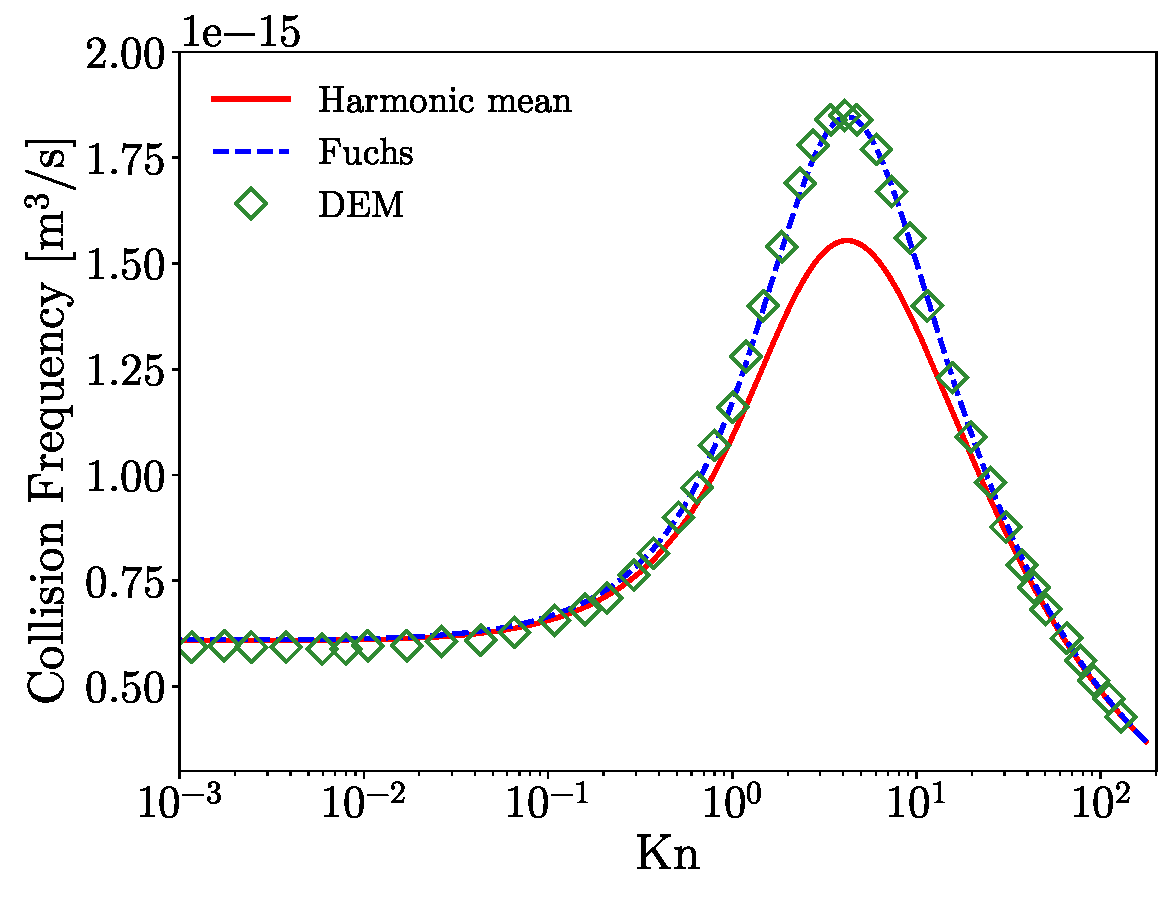
\includegraphics[width=0.45\textwidth]{Figures/Results/Validation/Kernel/kernel_valid.pdf}};
		\draw (-0.33, 1.11) node {\footnotesize{\cite{goudeli2015coagulation}}};
	\end{tikzpicture}
	\caption{The comparison of collision frequency, $\beta$, obtained by omnisoot using harmonic mean (red solid line) and Fuchs interpolation (green dashed line) with DEM results (symbols)~\citep{goudeli2015coagulation}}
	\label{fig:kernelvalid} 
\end{figure}

%\begin{figure}[!htbp]
%	\centering
%	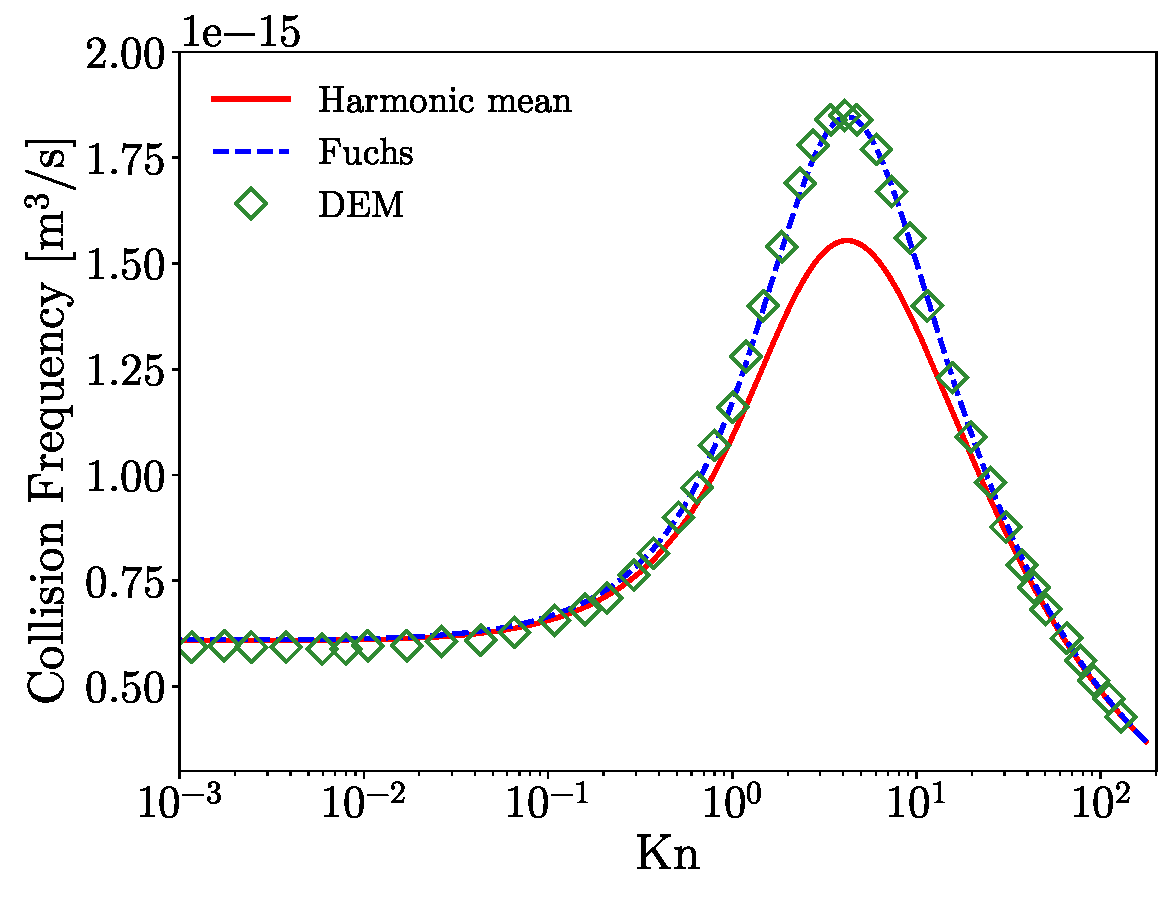
\includegraphics[width=0.55\textwidth]{Figures/Results/Validation/Kernel/kernel_valid.pdf}
%	\caption{The comparison of collision frequency, $\beta$, obtained by omnisoot using harmonic mean (red solid line) and Fuchs interpolation (green dashed line) with DEM results (symbols)~\citep{goudeli2015coagulation}}
%	\label{fig:kernelvalid}
%\end{figure} 


\section{The Effect of Excluding Five-membered Rings}

\begin{figure}[H]
	\centering
	\begin{tikzpicture}
		\draw (0, 0) node[inner sep=0] 	{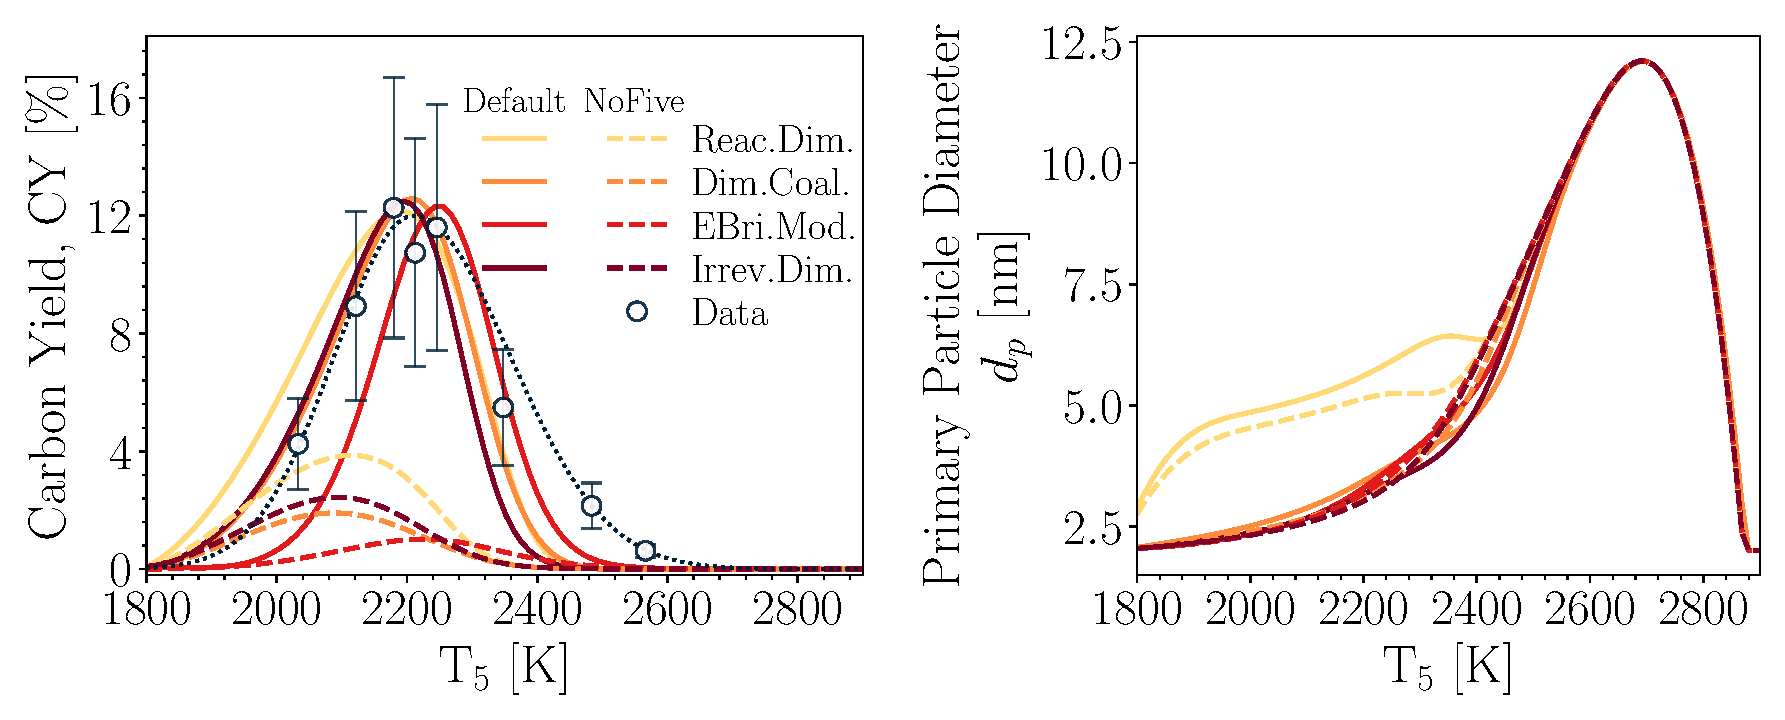
\includegraphics[width=0.8\textwidth]{Figures/Results/Shocktube/Agafonov2016_cpr/carbon_yield_dp_spc_combined.pdf}};
		\draw (-0.55, 0.29) node {\scriptsize{\cite{agafonov2016unified}}};
		%\draw (2.42, -0.23) node {\scriptsize{\cite{agafonov2016unified}}};
	\end{tikzpicture}
	\caption{The soot carbon yield, CY, at $t=$1.5 ms (a) and primary particle diameter, $d_p$ (b) obtained using the default soot precursors listed in Table~\ref{tab:precursors_list} (denoted by solid line and labeled as ``Default") compared with the same results when five-membered ring PAHs  excluded from soot precursors (denoted by dashed line and labeled as ``NoFive"). Both cases were obtained using Caltech mechanism and the same equal adjustment factors. The dashed line was added to show the trend in the measurements~\citep{agafonov2016unified}.}
	\label{fig:shockagof_yieldspc_cpr} 
\end{figure}



